\documentclass{standalone}
\usepackage{tikz}
\usepackage{calc}
\usepackage{pgffor}
\usetikzlibrary{patterns}
\begin{document}
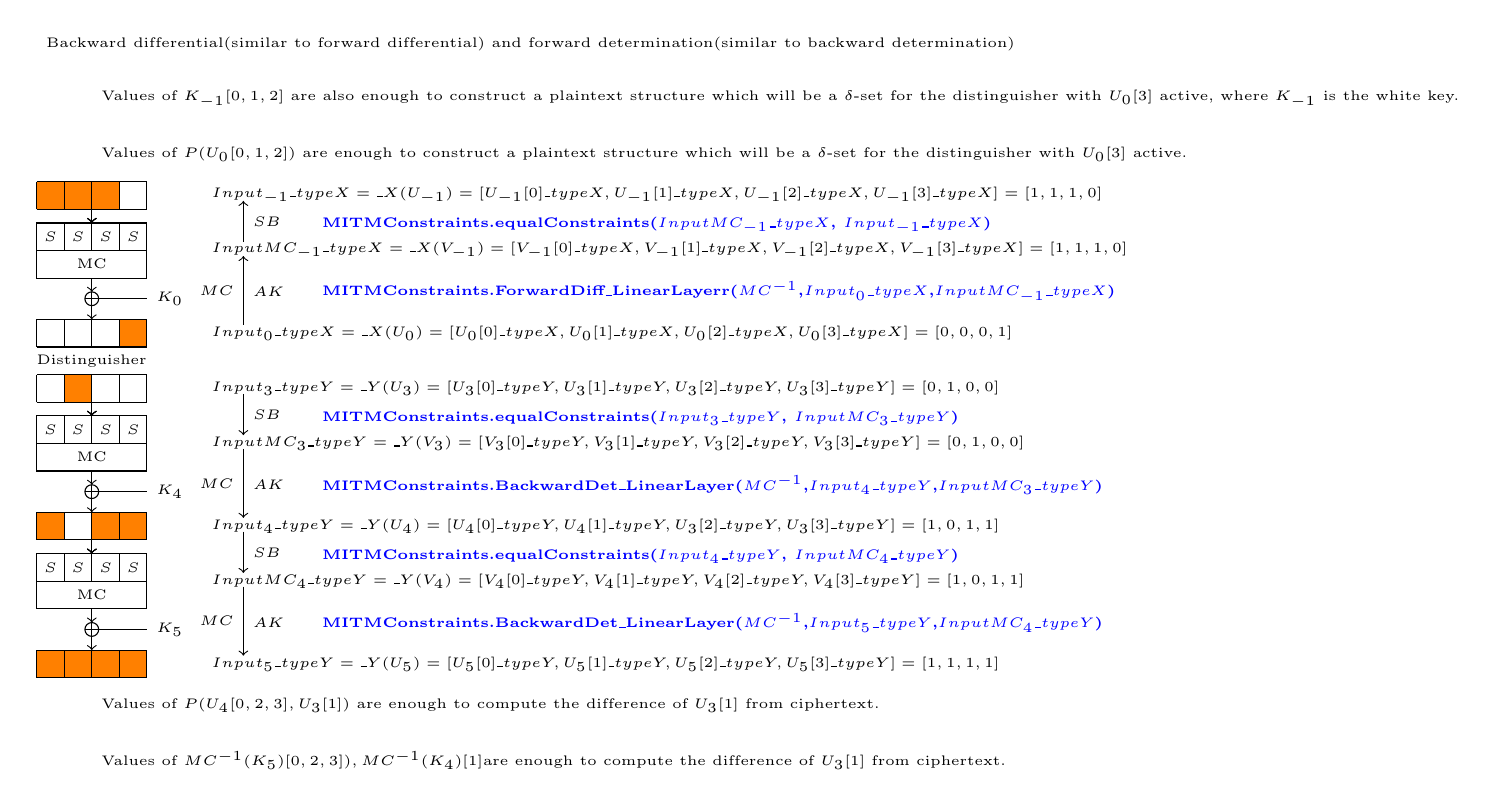
\begin{tikzpicture}[scale=0.35]
\begin{scope}[yshift = -5cm]
\fill[orange](3,0) rectangle+(1,1);
\end{scope}
\begin{scope}[yshift = 0cm]
\fill[orange](0,0) rectangle+(1,1);
\fill[orange](1,0) rectangle+(1,1);
\fill[orange](2,0) rectangle+(1,1);
\end{scope}
\begin{scope}[yshift = -7cm]
\fill[orange](1,0) rectangle+(1,1);
\end{scope}
\begin{scope}[yshift = -12cm]
\fill[orange](0,0) rectangle+(1,1);
\fill[orange](2,0) rectangle+(1,1);
\fill[orange](3,0) rectangle+(1,1);
\end{scope}
\begin{scope}[yshift = -17cm]
\fill[orange](0,0) rectangle+(1,1);
\fill[orange](1,0) rectangle+(1,1);
\fill[orange](2,0) rectangle+(1,1);
\fill[orange](3,0) rectangle+(1,1);
\end{scope}
\begin{scope}[yshift =0 cm]
\draw (0,0) grid +(4,1);
\foreach \y in {0,1,2,3}{\draw[->](2,0)--+(0,-0.5);
\draw(\y,-1.5) rectangle node{\tiny{$S$}} +(1,1);
}
\draw (0,-2.5) rectangle node{\tiny{MC}} +(4,1);
\draw[->] (2,-2.5)--+(0,-0.5);
\draw (1.75,-3.25)--+(0.5,0);
\draw (2,-3.25) circle (0.25);
\draw (4,-3.25) --(2.25,-3.25);
\node[right] at (4,-3.25) {\tiny{$K_0$}};
\draw[->](2,-3)--+(0,-1);
\end{scope}
\draw(0,-5) grid +(4,1);
\node at (2,-5.5){\tiny{Distinguisher}};
\begin{scope}[yshift =-7 cm]
\draw (0,0) grid +(4,1);
\foreach \y in {0,1,2,3}{\draw[->](2,0)--+(0,-0.5);
\draw(\y,-1.5) rectangle node{\tiny{$S$}} +(1,1);
}
\draw (0,-2.5) rectangle node{\tiny{MC}} +(4,1);
\draw[->] (2,-2.5)--+(0,-0.5);
\draw (1.75,-3.25)--+(0.5,0);
\draw (2,-3.25) circle (0.25);
\draw (4,-3.25) --(2.25,-3.25);
\node[right] at (4,-3.25) {\tiny{$K_4$}};
\draw[->](2,-3)--+(0,-1);
\end{scope}
\begin{scope}[yshift =-12 cm]
\draw (0,0) grid +(4,1);
\foreach \y in {0,1,2,3}{\draw[->](2,0)--+(0,-0.5);
\draw(\y,-1.5) rectangle node{\tiny{$S$}} +(1,1);
}
\draw (0,-2.5) rectangle node{\tiny{MC}} +(4,1);
\draw[->] (2,-2.5)--+(0,-0.5);
\draw (1.75,-3.25)--+(0.5,0);
\draw (2,-3.25) circle (0.25);
\draw (4,-3.25) --(2.25,-3.25);
\node[right] at (4,-3.25) {\tiny{$K_5$}};
\draw[->](2,-3)--+(0,-1);
\end{scope}
\draw (0,-17) grid +(4,1);


\begin{scope}[yshift = 0cm, xshift = 6cm]
\node[right] at (0, 0.5) {\tiny{$Input_{-1}\_typeX = \_X(U_{-1}) = [U_{-1}[0]\_typeX,U_{-1}[1]\_typeX,U_{-1}[2]\_typeX,U_{-1}[3]\_typeX]=[1,1,1,0]$}};

\draw[->] (1.5, -1.2)-- node[right] {\tiny{$SB$}} +(0,
  1.5);
\node[right] at (4, -0.6) {\textbf{\textcolor{blue}{\tiny{MITMConstraints.equalConstraints($InputMC_{-1}\_typeX$, $Input_{-1}\_typeX$)}}}};

\node[right] at (0,-1.5) {\tiny{$InputMC_{-1}\_typeX = \_X(V_{-1}) = [V_{-1}[0]\_typeX,V_{-1}[1]\_typeX,V_{-1}[2]\_typeX,V_{-1}[3]\_typeX]=[1,1,1,0]$}};

\draw[->] (1.5, -4.2)-- node[left] {\tiny{$MC$}} +(0,2.5);
\node[right] at (1.5,-3) {\tiny{$AK$}};
\node[right] at (4, -3) {\textbf{\textcolor{blue}{\tiny{MITMConstraints.ForwardDiff\_LinearLayerr($MC^{-1}$,$Input_0\_typeX$,$InputMC_{-1}\_typeX$)}}}};

\node[right] at (0,-4.5) {\tiny{$Input_0\_typeX = \_X(U_0) = [U_0[0]\_typeX,U_0[1]\_typeX,U_0[2]\_typeX,U_0[3]\_typeX]=[0,0,0,1]$}};
\end{scope}


\begin{scope}[yshift = -7 cm, xshift = 6cm]
\node[right] at (0, 0.5) {\tiny{$Input_3\_typeY = \_Y(U_3) = [U_3[0]\_typeY,U_3[1]\_typeY,U_3[2]\_typeY,U_3[3]\_typeY]=[0,1,0,0]$}};

\draw[->] (1.5, 0.3)-- node[right] {\tiny{$SB$}} +(0,-1.5);
\node[right] at (4, -0.6) {\textbf{\textcolor{blue}{\tiny{MITMConstraints.equalConstraints($Input_3\_typeY$, $InputMC_3\_typeY$)}}}};

\node[right] at (0,-1.5) {\tiny{$InputMC_3\_typeY = \_Y(V_3) = [V_3[0]\_typeY,V_3[1]\_typeY,V_3[2]\_typeY,V_3[3]\_typeY] =[0,1,0,0]$}};

\draw[->] (1.5, -1.7)-- node[left] {\tiny{$MC$}} +(0,-2.5);
\node[right] at (1.5,-3) {\tiny{$AK$}};
\node[right] at (4, -3) {\textbf{\textcolor{blue}{\tiny{MITMConstraints.BackwardDet\_LinearLayer($MC^{-1}$,$Input_4\_typeY$,$InputMC_3\_typeY$)}}}};

\node[right] at (0,-4.5) {\tiny{$Input_4\_typeY = \_Y(U_4) = [U_4[0]\_typeY,U_4[1]\_typeY,U_3[2]\_typeY,U_3[3]\_typeY]=[1,0,1,1]$}};

\end{scope}


\begin{scope}[yshift = -12 cm, xshift = 6cm]


\draw[->] (1.5, 0.3)-- node[right] {\tiny{$SB$}} +(0,-1.5);
\node[right] at (4, -0.6) {\textbf{\textcolor{blue}{\tiny{MITMConstraints.equalConstraints($Input_4\_typeY$, $InputMC_4\_typeY$)}}}};

\node[right] at (0,-1.5) {\tiny{$InputMC_4\_typeY = \_Y(V_4) = [V_4[0]\_typeY,V_4[1]\_typeY,V_4[2]\_typeY,V_4[3]\_typeY] =[1,0,1,1]$}};

\draw[->] (1.5, -1.7)-- node[left] {\tiny{$MC$}} +(0,-2.5);
\node[right] at (1.5,-3) {\tiny{$AK$}};
\node[right] at (4, -3) {\textbf{\textcolor{blue}{\tiny{MITMConstraints.BackwardDet\_LinearLayer($MC^{-1}$,$Input_5\_typeY$,$InputMC_4\_typeY$)}}}};

\node[right] at (0,-4.5) {\tiny{$Input_5\_typeY = \_Y(U_5) = [U_5[0]\_typeY,U_5[1]\_typeY,U_5[2]\_typeY,U_5[3]\_typeY]=[1,1,1,1]$}};

\end{scope}

\begin{scope}[yshift = -18cm]
\node[right] at (2,0) {\tiny{Values of $P(U_4[0,2,3],U_3[1])$ are enough to compute the difference of $U_3[1]$ from ciphertext.}};
\end{scope}

\begin{scope}[yshift = 0 cm]
\node[right] at (2,2) {\tiny{Values of $P(U_0[0,1,2])$ are enough to construct a plaintext structure which will be a $\delta$-set for the distinguisher with $U_0[3]$ active.}};
\end{scope}

\begin{scope}[yshift = 2 cm]
\node[right] at (2,2) {\tiny{Values of $K_{-1}[0,1,2]$ are also enough to construct a plaintext structure which will be a $\delta$-set for the distinguisher with $U_0[3]$ active, where $K_{-1}$ is the white key.}};
\end{scope}


\begin{scope}[yshift = -20 cm]
\node[right] at (2,0) {\tiny{Values of $MC^{-1}(K_5)[0,2,3]), MC^{-1}(K_4)[1]$are enough to compute the difference of $U_3[1]$ from ciphertext.}};
\end{scope}

\begin{scope}[yshift = 6 cm]
\node[right] at (0,0) {\tiny{Backward differential(similar to forward differential) and forward determination(similar to backward determination)}};
\end{scope}

\end{tikzpicture}
\end{document}